% Součást skript na Datové struktury. Viz main.tex
\markright{$ $Id$ $}


\chapter{Binární vyhledávací stromy}
\label{bvs}
% --------------------------------------------------------------------------
% by Vladimir Kotal, 2004


% ..........................................................................
\section{Obecně}
\label{bvs:obecne}

\begin{defn}
\emph{Binární vyhledávací strom} reprezentující množinu $S$ je takový 
binární strom, že 

\begin{enumerate}
\item každý vnitřní vrchol má dva syny, levého a pravého
\item existuje jednoznačná korespondence mezi vrcholy $S$ a vnitřními 
vrcholy stromu
\item pro každý vnitřní vrchol $v$ platí, že vnitřní vrcholy $v$ podstromu 
jeho levého syna reprezentují prvky menší než reprezentuje $v$ a vnitřní 
vrcholy v podstromu jeho pravého syna reprezentují prvky větší než 
reprezentuje vrchol $v$.
\end{enumerate}
\end{defn}

\begin{pozn}
Nechť

$$
S = \{ s_1 < s_2 < ... < s_n \}
$$
$$
s_0 = - \infty, s_{n+1} = \infty
$$

Pak $i$-tý list (ve smyslu zleva doprava) reprezentuje interval 
$<s_{i-1}, s_i>$.
\end{pozn}

\begin{priklad}
Nechť $S = \{ 1, 7, 12, 15, 24, 81 \}$. Binární vyhledávací strom
reprezentující množinu $S$ je na obr.~\ref{fig.bvs.example}.
\mnote{Strom na obr.~\ref{fig.bvs.example} není možná nejlepší příklad,
protože BVS mohou vypadat více nepravidelně - na rozdíl od haldy
\emph{nemusí} mít všechny uzly umístěny co možná nejvíce "vlevo".}

\begin{figure}[!htb]
\centering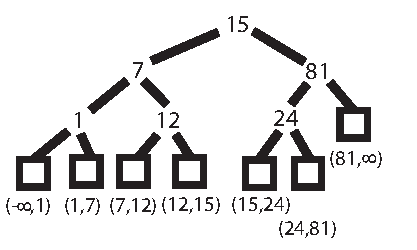
\includegraphics{pics/bvs}
\caption{Příklad binárního vyhledávacího stromu}
\label{fig.bvs.example}
\end{figure}

\end{priklad}

\begin{pozn}
V listech máme jen intervaly, každý vrchol implicitně určuje tyto
intervaly. (viz obr.~\ref{fig.bvs.example}) Tato vazba je jednotlivými
operacemi udržována.
\end{pozn}

\subsection{Algoritmus MEMBER}

\begin{algorithm}[!htb]
\caption{MEMBER pro binární vyhledávací stromy}
\label{alg:btr.mem}
\begin{algorithmic}
\STATE $t \leftarrow$ kořen
\WHILE {$t$ \text{není list a zároveň} $t$ \text{nereprezentuje} $x$} 
\IF {$x >$ \text{prvek reprezentovaný} $t$}
  \STATE $t \leftarrow$ pravý syn
\ELSE 
   \STATE $t \leftarrow$ levý syn $t$
\ENDIF
\ENDWHILE
\end{algorithmic}
\end{algorithm}


\subsection{Algoritmus INSERT}

\mnote{tohle je pouze pokus o alg. 
XXX dopsat podle nějakého důvěryhodného zdroje !}
\begin{enumerate}
  \item najdi list kam patří $x$ ($x_{i-1} < x < x_i$)
  \item udělej z něj vnitřní vrchol s hodnotou $x$
  \item přidej mu dva syny s intervaly $<x_{i-1}, x> , <x, x_i>$
  \item uprav strukturální podmínku na strom
\end{enumerate}


\subsection{Algoritmus DELETE}

DELETE(x) provedeme následovně: 

\begin{enumerate}
  \item nalezneme $x$ (vrchol reprezentující $x$)
  \item pokud jeden jeho syn je list, pak odstraníme vrchol + syna, který je
    list, druhý syn nahradí odstraněný vrchol
\mnote{co když oba synové jsou listy ?}
  \item pokud žádný jeho syn není list, pak:
    nalezneme vrchol $u$, reprezentující nejmenší prvek v $S$ větší než $x$.
    levý syn tohoto vrcholu je list.
    přemístíme prvek reprezentovaný tímto vrcholem do vrcholu
    reprezentujícího $x$ odstraníme $u$ a jeho levého syna, pravého syna
    $u$ dáme na místo $u$.
\end{enumerate}

Jak nalezneme vrchol reprezentující nejmenší prvek v $S$ větší než $x$ ?
Jsme ve vrcholu $t$ reprezentujícím $x$ a hledáme vrchol $u$:
\begin{algorithmic}
\STATE $u \leftarrow$ pravý syn $t$
\WHILE {\text{levý syn} $u \neq list$}
   \STATE $u \leftarrow$ levý syn $u$
\ENDWHILE
\end{algorithmic}

Čas pro operace MEMBER, INSERT a DELETE v binárním vyhledávacím stromě je
\\
$O(\text{délka stromu}) = O(\text{výška stromu})$.

% --------------------------------------------------------------------------
\section{Optimální binární vyhledávací stromy}

Budeme chtít reprezentaci binárního vyhledávacího stromu takovou, že 
bude optimalizovaná vzhledem k operaci MEMBER za předpokladu, že známe
pravděpodobnost provedení této operace na jednotlivé vrcholy stromu.

\subsection{Co je to optimální binární vyhledávací strom}

Prvky jsou uloženy ve vnitřních vrcholech stromu. 
Listy jsou intervaly $(-\infty, x_1)$, $(x_1, x_2)$, 
$\ldots$, $(x_n, \infty)$. Listy nemusíme implicitně
ve stromě zaznamenávat.
U optimálních stromů dále předpokládáme, že známe pravděpodobnosti 
operací $Access(x)$. 

\subsection{Algoritmus konstrukce}

Dána množina $S = \{x_1 < x_2 < ... < x_n \}$, provádí se pouze operace
MEMBER(x) a jsou dány pravděpodobnosti 
$\alpha_1, ..., \alpha_n, \beta_0, ..., \beta_n$, kde 
\begin{itemize}
\mnote{P značí pravděpodobnost}
\item $\alpha_i = P($prováděla se operace $MEMBER(x_i))$
\item $\beta_i = P($prováděla se operace $MEMBER(x)$ pro 
   $x \in <x_i, x_{i+1}>)$
\end{itemize}

kde $x_0 = - \infty, x_{n+1} = \infty$.
\par
Tedy jsou dány pravděpodobnosti přístupu k vnitřním vrcholům a k listům.
\par

Chceme nalézt binární vyhledávací strom reprezentující $S$ takový, že
operace MEMBER má nejmenší očekávaný čas.
\par
Očekávaný čas operace MEMBER je $\sum_{i=1}^{n} \alpha_i(a_i + 1) +
\sum_{i=0}^{n} \beta_i b_i$, kde 
\mnote{očekávaná hodnota = střední hodnota náhodné veličiny; n.v. s
diskrétním rozdělením má stř. hodnotu $\sum x_i p_i$}
$a_i$ je hloubka prvku reprezentujícího prvek $x_i$, $b_i$ je hloubka
listu reprezentujícího interval $<x_i, x_{i+1}>$.
\par

\subsubsection{Zobecníme úlohu:}

\mnote{XXX sjednotit indexy a závorky - buď $c(i,j)$ nebo $c_{i,j}$}
Dána množina $S = \{x_1 < x_2 < ... < x_n \}$ a ohodnocení $\alpha_i$ prvku
$x_i$ a $\beta_i$ intervalu $(x_i,x_{i+1})$.
Chceme zkonstruovat binární vyhledávací strom T reprezentující S takový,
že $hod(T)= \sum_{i=1}^{n} \alpha_i(a_i + 1) + \sum_{i=0}^{n} \beta_i b_i$
je minimální. \\
T je pak optimální binární vyhledávací strom.
Pro $1 \leq i \leq j \leq n$, $U_{i,j}$ je úloha nalézt optimální binární
vyhledávací strom pro $S_{i,j} = {x_i < x_{i+1} < ... < x_j}$ a hodnoty 
$\alpha_i, \alpha_{i+1}, ..., \alpha_j, \beta_{i-1}, \beta_i, ..., \beta_j$.

\par
\begin{pozorov}
\label{obvs-poz1}
% Pozorování 1: 
Nechť T je strom reprezentující množinu $S_{i,j}$ a kořen T
hodnotí prvek $x_k$ pro $i \leq k \leq j$. Nechť $T_l$ je podstrom levého
syna kořene, $T_p$ je podstrom pravého syna kořene. Pak: \\
$hod(T) = hot(T_l) + hod(T_p) + \sum_{l=i}^{j} \alpha_l + \sum_{l=i-1}^{j}
\beta_l$ \\
$T_l$ reprezentuje množinu $S_{i,k-1}$ a $T_p$ reprezentuje množinu $S_{k+1,j}$.
\end{pozorov}

\par
\begin{pozorov}
% Pozorování 2: 
Nechť platí předpoklady pozorování
% Pozorování 1 
\ref{obvs-poz1}
a nechť T je optimální
binární vyhledávací strom pro $S_{i,j}$. Pak $T_l$ je optimální
binární vyhledávací strom pro $S_{i,k-1}$ a $T_p$ je optimální
binární vyhledávací strom pro $S_{k+1,j}$.
\end{pozorov}

\par
\begin{pozorov}
% Pozorování 3: 
Když známe $hod(T_{k,k'})$ pro opt. bin. vyhl. strom
reprezentující množinu $S_{k,k'}$ kde $i \leq k \leq k' \leq j$ a $k'-k <
j-i$, pak $hod(T_{i,j})$ pro opt. bin. vyhl. strom je \\
$$
\sum_{l=i}^{j} \alpha_l + \sum_{l=i-1}^{j} \beta_l + min\{hod(T_{i,k-1}) +
hod(T_{k+1,j}), i \leq k \leq j\}
$$
Když 
$$
hod(T_{i,k-1}) + hod(T_{k+1,j})
\leq min\{hod(T_{i,k'-1}) + hod(T_{k'+1,j}), i \leq k' \leq j\}
$$
pak $\exists$ opt. bin. vyhl. strom pro $S_{i,j}$,
jehož kořen reprezentuje $x_k$.
\end{pozorov}

\par
Systematicky spočítáme $w_{i,j} = \sum_{l=i}^{j} \alpha_l + \sum_{l=i-1}^{j}
\beta_l$ pro všechny $1 \leq i \leq j \leq n$. Inicializujeme matice H,K
typu $n x n, H = K = 0$.
\mnote{XXX typu n krat n}

\begin{algorithmic}
\FOR {i=1,2,...,n} 
  \STATE $H_{i,i} = w_{i,i}, K_{i,i} = i$
\ENDFOR
\end{algorithmic}

$H_{i,j}$ pro $i \leq j$ bude $H_{i,j} = hod(T_{i,j})$ pro opt. bin. vyhl.
strom reprezentující $S_{i,j}$ a $K_{i,j}$ bude index prvku
reprezentovaného v kořeni $T_{i,j}$.

\begin{algorithm}[!htb]
\caption{Výpočet matic H, K}
\label{alg:obvs.puv}
\begin{algorithmic}
\FOR {every $i=1,2,..,n$}
  \STATE $H_{i,i} = w_{i,i}, K_{i,i} = i$
\ENDFOR
\STATE $j = 1$
\WHILE {$j < n$}
  \STATE $i = 1$
  \WHILE {$i+j \leq n$}
    \STATE $m = i, hod = H_{i+1,j}$ (1)
    \STATE $k = i+1$  (2)
    \WHILE {$k \leq i+j$ (3)} 
      \IF {$hod > H_{i,k-1} + H_{k+1,i+j}$}
        \STATE $hod = H_{i,k-1}+H_{k+1,i+j}$
	\STATE $m = k$
      \ENDIF
      \STATE $k = k + 1$
    \ENDWHILE
    \STATE $H_{i,i+j} = hod + w_{i,i+j}, K_{i,i+j} = m, i = i + 1$
  \ENDWHILE
  \STATE $j = j + 1$
\ENDWHILE
\end{algorithmic}
\end{algorithm}

\begin{theorem}
Uvedený algoritmus \ref{alg:obvs.puv} spočítá korektně matice $H$ a $K$ 
v čase $O(n^3)$ a vyžaduje $O(n^2)$ paměti.
\end{theorem}

$K_{i,j} \leq K_{i,j+1} \leq K_{i+1,j+1}$

\mnote{XXX obr. matice}

\subsubsection{Konstrukce opt. bin. vyhl, stromu ze znalosti matice $K$}
\begin{itemize}
\item kořen stromu bude $x_{K(1,n)}$.
\item podstrom levého syna bude optim. strom pro $S_{1,K(1,n)-1}$
\item podstrom pravého syna bude optim. strom pro $S_{K(1,n)+1,n}$
\end{itemize}

To nám dává rekurzivní algoritmus pro výstavbu opt. bin. vyhl. stromu z
matice $K$, strom takto zkonstruujeme v čase $O(n)$.


% --------------------------------------
\subsection{Snížení složitosti z kubické na kvadratickou}

XXX sloučit s částí předch subsekce

Chceme snížit ryhchlost konstrukce opt. bin. vyhl. stromu z kubické na
kvadratickou. Pro tento úkol použijeme \emph{kvadratické programování}. 
Pomocí této techniky lze modifikovat algoritmus pro konstrukci optimální
BVS tak, že bude mít místo složitosti $O(n^3)$ složitost $O(n^2)$.

Algoritmus~\ref{alg:obvs.puv} pro výpočet $H$ a $K$ jsme modifikovali tak,
že řádky (1),(2),(3) jsme nahradili řádky (1'),(2'),(3'). Tím vznikl
algoritmus~\ref{alg:obvs.modif}.

\begin{algorithm}[!htb]
\caption{Modifikovaný algoritmus pro výpočet matic H, K}
\label{alg:obvs.modif}
\begin{algorithmic}
\FOR {every $i=1,2,..,n$}
  \STATE $H_{i,i} = w_{i,i}, K_{i,i} = i$
\ENDFOR
\STATE $j = 1$
\WHILE {$j < n$}
  \STATE $i = 1$
  \WHILE {$i+j \leq n$}
    \STATE $m = K_{i,i} + j, hod = H_{i,m-1} + H_{m+i,i+j}$ (1')
    \STATE $k = K_{i,i+j} + 1$ (2') 
    \WHILE {$k \leq K_{i+1,j+1}$ (3')} 
      \IF {$hod > H_{i,k-1} + H_{k+1,i+j}$}
        \STATE $hod = H_{i,k-1}+H_{k+1,i+j}$
	\STATE $m = k$
      \ENDIF
      \STATE $k = k + 1$
    \ENDWHILE
    \STATE $H_{i,i+j} = hod + w_{i,i+j}, K_{i,i+j} = m, i = i + 1$
  \ENDWHILE
  \STATE $j = j + 1$
\ENDWHILE
\end{algorithmic}
\end{algorithm}

Modifikovaný algoritmus: Třetí vnořený cyklus vyžaduje čas 
$O(K_{i+1,j+1} - K_{i,j})$. Tedy druhý vnořený cyklus vyžaduje čas 
$O(K_{2,2+j} - K_{1,1+j} + K_{3,3+j} - K_{2,2+j} + K_{4,4+j} - K_{3,3+j} +
... + K_{n-j,n} - K_{n-j-1,n-1}) = O(K_{n-j,n}) = O(n)$.

\begin{theorem}
Za předpokladu $K_{i,j} \leq K_{i,j+1} \leq K_{i+1,j+1}$ pro každé 
$1 \leq i \leq j \leq n - 1$ modifikovaný algoritmus korektně spočítá
matice $H$ a $K$ v čase $O(n^2)$ a vyžaduje paměť $O(n^2)$.
\end{theorem}



\par
Vstup: dána čísla $w(i,j), 1 \leq i \leq j \leq n$\\
Výstup: definujeme  $c(i,j) = $
 \(
 \begin{cases}
 	0
		&\text{pro } i=j, \text{kde } i = 1,2,..., n\\
	w(i,j) + min\{c(i,k-1) + c(k,j),
		i < k \leq j\}&\text{pro } i \neq j
 \end{cases}
 \)

Úkolem je tedy nalézt čísla $c(i,j)$.
Čísla $c(i,j)$ budou tvořit výstup algoritmu. Když použijeme modifikaci
algoritmu pro hledání opt. bin. vyhl. stromu, pak spočítáme $c(i,j)$ v
čase $O(n^3)$.
\par

\begin{defn}
$K(i,j) = min\{l, l=i+1, ..., j \text{ a platí }
c(i,l-1) + c(l,j) \leq c(i,k-1) + c(k,j) \forall k = i+1, ...,j\}$ 
\end{defn}

Když $K(i,j) \leq K(i,j+1) \leq K(i+1,j+1)$ pro $i \leq j$, pak lze použít
algoritmus vyžadující čas $O(n^2)$. (tj. můžeme použít rychlejší
modifikaci algoritmu pro hledání opt. bin. vyhl. stromu a
spočítáme $c(i,j)$ v čase $O(n^2)$)

\begin{pozn}
Vztah kvadratického programování a hledání opt. bin. vyhl. stromu:
Položme $w(i,j) = \sum_{l=i}^{j} \alpha_l + \sum_{l=i-1}^{j} \beta_l$, pak
$c(i,j) = H_{i+1,j}$.
\end{pozn}

\par
Chceme ukázat, že když platí

\begin{itemize}
\item (A) $w(i,j) \leq w(i',j')$ pro $i' \leq i \leq j \ leq j'$ 
\item (B) $w(i,j) + w(i',j') \leq w(i,j') + w(i',j)$ pro 
$i \leq i' \leq j \ leq j'$ 
\end{itemize}

pak platí 
$K(i,j) \leq K(i,j+1) \leq K(i+1,j+1)$ pro $1 \leq i \leq j$.

\begin{lemma}
Za uvedených předpokladů platí \\
$c(i,j) + c(i',j') \leq c(i,j') + c(i',j)$ pro $i \leq i' \leq j \ \leq j'$ 
\end{lemma}

\begin{proof}
indukcí dle $j'-i$: \\
platí: když $i = i'$ nebo $j = j'$, pak triviálně platí \\
$c(i,j) + c(i',j') \leq c(i,j') + c(i',j)$ 

iniciální krok: když $j'-i \leq 0$, pak platí buď $i = i'$ nebo $j = j'$. \\
indukční krok: předpokládejme, že nerovnost platí, když $j'-i < n$ a
nechť $j'-i = n$, kde $n \geq 2$.

\begin{enumerate}
% 1)
\item $j = i'$ pak máme dokázat, že \\
$c(i,j) + c(j,j') \leq c(i,j')$. označme $K(i,j') = l$.

\begin{enumerate}
\item
(1a)
$l \leq j$ pak $c(i,j) + c(j,j') \stackrel{\text{z def } c(i,j)}{\leq} w(i,j) + c(i,l-1) + c(l,j)+ c(j,j')
\stackrel{\text{z (A) a ind. předp.}}{\leq} w(i,j') + c(i,l-1) = c(i,j)$  \\
víme, že $i < l \leq j$, tedy $j'-l < j'-i$. \\
$\Rightarrow$ (1a) platí.
\item
(1b) $l \geq j$, důkaz stejný jako pro 1a. \\
$\Rightarrow$ 1 platí.
\end{enumerate}

% 2)
\item $j > j'$ \\
označme $k = K(i,j'), l = K(i',j)$ \\

\begin{enumerate}
\item (2a) $l \leq k$, pak $i' < l < \leq j, i < k < j \leq j'$ \\
\begin{align*}
&c(i,j) + c(i',j') \\
\leq &w(i,j) + c(i,l-1) + c(l,j) + w(i',j') + c(i',k-1) + c(k,j') \\
= &w(i,j) + w(i',j') + c(i,l-1) + c(i',k-1) + c(l,j) + c(k,j') \\
\stackrel{\text{podle (B)}}{\leq} 
&w(i,j') + w(i',j) + c(i,k-1) + c(i',l-1) + c(l,j) + c(k,j') =
\end{align*}
\mnote{$c(i,k-1) + c(i',l-1)$ jsme dostali z ind. předp.}

víme, že $i \leq i' \leq l-1 \leq k-1$ a $k-1-i < j'-i$. \\
Potom 

\begin{align*}
= &w(i,j') + c(i,k-1) + c(k,j') + w(i',j) + c(i,l-1) c(l,j) \\
= &c(i,j') + c(i',j)
\end{align*}

\item (2b) $k \leq l$ důkaz je analogický jako pro (2a).
\end{enumerate}
$\Rightarrow$ 2 platí.
\end{enumerate}
$\Rightarrow$ lemma je dokázané.
\end{proof}

\begin{lemma}
Když $c(i,j) + c(i',j') \leq c(i,j') + c(i',j)$ pro $i \leq i' \leq j \leq
j'$, pak platí \\
$K(i,j) \leq K(i,j+1) \leq K(i+1,j+1)$
\end{lemma}

\begin{proof}
Ukážeme, že platí $K(i,j) \leq K(i,j+1)$, důkaz druhé nerovnosti je
analogický. \\
Abychom dokázali $(i,j) \leq K(i,j+1)$, tak stačí ukázat, že platí \\
$c(i,k-1) + c(k,j) <  c(i,k'-1) + c(k',j)$ pak
$c(i,k-1) + c(k,j+1) <  c(i,k'-1) + c(k',j+1)$ pro $i < k' < k \leq j$.

požadovaná nerovnost plyne z této nerovnosti: \\
\begin{align*}
&c(i,k'-1) + c(k',j) - c(i,k-1) - c(k,j) \\
\stackrel{c(i,k'-1) > 0}{\leq} 
&c(i,k'-1) + c(k',j+1) - c(i,k-1) - c(k,j+1)
\end{align*}

skončili jsme s triky, upravíme nerovnost a vyjde to: \\
\begin{align*}
&c(i,k'-1) + c(k',j) + c(i,k-1) + c(k,j+1) \\
\leq &c(i,k'-1) + c(k',j+1) + c(i,k-1) + c(k',j+1) 
\end{align*}

$c(k',j) + c(k,j+1) \leq c(k',j+1) + c(k,j)$
platí $k' < k \leq j \leq j+1$ ... nerovnost platí dle předpokladu
(položíme i = k', i'=k, j=j, j'=j+1)
\mnote{XXX pokud se divíte $j=j$, nedivte se, znamená to, že j z 1. části se
rovná j z druhé části :) chce to lepší značení}
\end{proof}


% --------------------------------------------------------------------------
\section{Skorooptimální binární vyhledávací stromy}

% Jenom že existují, lineární konstrukce. Aha --- viz cvičení.

% \mnote{referát by Ladislav Strojil}
\newtheorem{fakt}{Fakt}

\renewcommand{\labelenumi}{\arabic{enumi})}
\newcommand{\oops}[1]{\textbf{#1}}

% tady jsem z referatu vytrhnul definici bin. opt. vyhr. stromu a presunul
% ji nahoru k bin. opt. vyhl. stromum
% V. Kotal, 2004

\begin{defn} Nechť $S=\{x_1 < x_2 < \ldots < x_n\}$ 
a nechť $\beta_i$ (resp. $\alpha_j$) je prav\-dě\-po\-dob\-nost operace 
$Access(a,S)$, kde $a=x_i$ (resp. $x_j < a < x_{j+1}$) pro $1 \leq i \leq n$ 
(resp. $0 \leq j \leq n$).
Potom $\beta_i\geq0$, $\alpha_i\geq0$ a $\sum{\beta_i}+\sum{\alpha_i}=1$. 
(2n+1)-tice $(\alpha_0,\beta_1,\alpha_1,\ldots,\beta_n,\alpha_n)$ se nazývá 
\emph{rozdělení (pravděpodobnosti) přístupu}.
\end{defn}

Strom potom konstruujeme rekurzí tak, aby \emph{průměrná vážená cesta} 
ve stro\-mě byla co nejkratší.
\par

Takový strom lze konstruovat pomocí rekurzivního výpočtu zkoušením všech 
kandidátů na kořen. To lze v čase $O(n^2)$, protože volba kořene jednoznačně určuje 
prvky pravého i levého podstromu (neboť se jedná o vyhledávací strom).
Takový strom lze konstruovat pomocí rekurzivního výpočtu zkoušením všech 
kandidátů na kořen. To lze v čase $O(n^2)$, protože volba kořene jednoznačně určuje 
prvky pravého i levého podstromu (neboť se jedná o vyhledávací strom).
\subsection{Aproximace optimálních stromů}

\par
Při konstrukci se budeme snažit volbou kořene podstromu rozdělit prvky na dvě stejně pravděpodobné množiny.

Uvažujme následující situaci. $S=\{x_1, x_2, x_3, x_4\}$ s pravděpodobnostmi pří\-stu\-pu
($\alpha_0$, $\beta_1$, $\alpha_1$, $\beta_2$, $\alpha_2$, $\beta_3$, $\alpha_3$, $\beta_4$, $\alpha_4$) = 
$(\frac{1}{6},\frac{1}{24},0,\frac{ 1}{8},0,\frac{ 1}{8},\frac{ 1}{8}, 0,\frac{ 5}{12})$.

\par
Doporučuji si představit uvedené body na reálné ose tak, že $\alpha_0$ je v bodě $0$, $\alpha_4$ v bodě $1$.

\par
Bod $\frac{1}{2}$ padne buď do $\beta_i$ nebo do $\alpha_j$ pro nějaké $i$, resp. $j$. V prvním případě zvolíme $x_i$ jako 
kořen stromu, jinak volíme mezi $x_j$ a $x_{j+1}$, podle toho, zda $\frac{1}{2}$ leží v levé nebo pravé polovině $\alpha_j$. 

\par
V našem případě volíme $x_3$ jako kořen stromu.

\par
Pro rozhodnutí o kořenu levého podstromu vrchol, který popsaným způ\-sobem odpovídá bodu $\frac{1}{4}$. Tento postup není totožný s postupem, 
kdy se bere bod $\frac{1}{2}$ v 
nově vzniklé podúloze, protože při konstrukci podstromu bychom zanedbali část intervalu $\alpha_3$.

\subsection{Podrobnější popis naznačené metody}

Nechť 
\begin{equation} 
s_0 = \frac{\alpha_0}{2} \\ s_i = s_{i-1} + \frac{\alpha_{i-1}}{2} + \beta_i + \frac{\alpha_i}{2}.
\end{equation}

\par
Uvědomte si, že $s_i$ jsou středy intervalů příslušejících "neúspěšnému
vy\-hle\-dá\-vá\-ní", tj. $(x_i,x_{i+1})$.

\par
Volání funkce $construct\_tree(0,n,0,1)$ vytvoří skoro optimální
vyhledávací strom dle popsané metody.

\ \newline
\oops{procedure} contruct\_tree(i,j,cut,l)

\emph{Poznámka: Předpokládáme, že parametry volané funkce splňují následující podmínky.}
\begin{enumerate}
\item $i$ a $j$ jsou celá čísla taková, že $0 \leq i < j \leq n$
\item $l$ je celé číslo, $l \geq 0$
\item $cut=\sum_{p=1}^{l-1}{x_p 2^{-p}}$, kde $x_p \in \{0, 1\}$ pro všechna $p$
\item $cut \leq s_i \leq s_j \leq cut + 2^{-l+1}$
\end{enumerate}
\emph{Volání $construct\_tree(i,j,,)$ vytvoří binární vyhledávací strom pro vrcholy $i+1, \ldots, j$ a listy $i, \ldots, j$.}

\oops{begin}

\ \ \ \oops{if} $i+1=j$ (případ A) \oops{return} kořen=j, levý list=i, pravý list=j;

\ \ \ \ \ \oops{else}

\ \ \ \ \ \ \ \ najdi k takové, že

\ \ \ \ \ \ \ \ 5) $i < k \leq j$

\ \ \ \ \ \ \ \ 6) $k = i + 1$ nebo $s_{k-1} \leq cut + 2^{-l}$

\ \ \ \ \ \ \ \ 7) $k = j$ nebo $s_{k} \geq cut + 2^{-l}$

\ \ \ \ \ \ \ \ \emph{Takové $k$ vždy existuje, protože parametry funkce splňují podmínku 4.}

\ \ \ \ \ \ \ \ \oops{if} $k = i + 1$ (případ B) \oops{return}

\ \ \ \ \ \ \ \ \ \ \ \ \ \ \ \ \ \ \ \ \ \ \ \ kořen=i+1

\ \ \ \ \ \ \ \ \ \ \ \ \ \ \ \ \ \ \ \ \ \ \ \ levý list=i

\ \ \ \ \ \ \ \ \ \ \ \ \ \ \ \ \ \ \ \ \ \ \ \ pravý list=\oops{construct\_tree}(i+1,j,cut+$2^{-l}$,l+1);

\ \ \ \ \ \ \ \ \oops{if} $k = j$ (případ C) \oops{return} 

\ \ \ \ \ \ \ \ \ \ \ \ \ \ \ \ \ \ \ \ \ \ \ \ kořen=j

\ \ \ \ \ \ \ \ \ \ \ \ \ \ \ \ \ \ \ \ \ \ \ \ levý list=\oops{construct\_tree}(i,j-1,cut,l+1)
	
\ \ \ \ \ \ \ \ \ \ \ \ \ \ \ \ \ \ \ \ \ \ \ \ pravý list=j;

\ \ \ \ \ \ \ \ \oops{if} $i + 1 < k < j$ (případ D) \oops{return}

\ \ \ \ \ \ \ \ \ \ \ \ \ \ \ \ \ \ \ \ \ \ \ \ kořen=k

\ \ \ \ \ \ \ \ \ \ \ \ \ \ \ \ \ \ \ \ \ \ \ \ levý list=\oops{construct\_tree}(i,k-1,cut,l+1)
	
\ \ \ \ \ \ \ \ \ \ \ \ \ \ \ \ \ \ \ \ \ \ \ \ pravý list=\oops{construct\_tree}(k,j,cut+$2^{-l}$,l+1);

\oops{end}


\begin{theorem}
Nechť $b_i$ je hloubka vrcholu $x_i$ a $a_j$ je hloubka listu $(x_j,x_{j+1})$ ve stromě $T_{BB}$ vytvořeném funkcí 
\oops{construct\_tree}(0,n,0,1). Potom

$b_i \leq \lfloor \log{1/\beta_i}\rfloor$, $a_j \leq \lfloor \log{1/\alpha_j}\rfloor + 2$ 
\end{theorem}

\begin{proof}
\emph{Věta říká, že hloubka vrcholu roste s klesající pravděpodobností přístupu k tomuto vrcholu.}

Plyne z následujících faktů.
\end{proof}

\begin{fakt}
Jestliže hodnoty parametrů funkce \oops{construct\_tree} splňují 
podmínky 1-4 a $i + 1 \neq j$, potom k splňující požadované podmínky existuje 
a hodnoty parametrů rekurzivních volání \oops{construct\_tree} splňuji 1-4.
\end{fakt}

\begin{proof} 
\ \par
Předpokládejme, že parametry splňují 1 -- 4 a $i + 1 \neq j$. 
Potom zřejmě platí $cut \leq s_j \leq cut + 2^{-l+1}$. Pro spor předpokládejme, 
že neexistuje neexistuje žádné $k$, $i < k \leq j$, pro které 
by platilo $s_{k-1} \leq cut+2^{-l}$ a $s_{k} \geq cut+2^{-l}$. 

Potom ovšem buď pro všechna $k$ taková, že $i < k \leq j$, 
platí $s_{k} < cut+2^{-l}$ nebo 
pro všechna $k$ taková, že $i < k \leq j$, platí $s_{k-1} > cut+2^{-l}$.

\par
V prvním případě $k = j$ odpovídá požadovaným podmínkám, 
v druhém jim odpovídá $k = i + 1$. Tedy $k$ vždy existuje.

\par
Zbývá ukázat, že nové parametry volání funkce splňují požadované 
pod\-mín\-ky. To ale plyne z toho, že $k$ splňuje 5-7 a  $i+1 \neq j$.
\end{proof}

\begin{fakt}
Hodnoty parametrů všech volání \oops{construct\_tree} splňují podmínky 1-4.
\end{fakt}
\begin{proof} 
Indukcí. \oops{construct\_tree}(0, n, 0, 1) splňuje 1-4 a pomocí předchozího faktu.
\end{proof}

Řekneme, že vrchol $h$ (resp. list $h$) je vytvořen voláním 
\oops{construct\_tree}(i, j, cut, l), jestliže $h = j$ (resp. $h =j$ nebo $h = i$) a 
byl proveden případ A, nebo $h = i + 1$ (resp. $h = i$) a byl proveden případ B, 
nebo $h = j$ a byl proveden případ C, nebo  $h = k$ 
a byl proveden případ D.

\par
Dále něchť $b_i$ je hloubka vrcholu $i$ a $a_j$ hloubka listu $j$ ve 
stromě vráceném $construct\_tree(0,n,0,1)$.

\begin{fakt}
Je-li vrchol $h$ (resp. list $h$) vytvořen voláním 
$construct\_tree(i,j,cut,l)$, potom $b_h + 1 = l$ (resp. $a_h = l$).
\end{fakt}
\begin{proof}
Indukcí podle $l$. 
\end{proof}
\begin{fakt}
Je-li vrchol $h$ (resp. list $h$) vytvořen voláním 
$construct\_tree(i,j,cut,l)$, potom $\beta_h \leq 2^{-l+1}$ (resp. $\alpha_h \leq 2^{-l+2}$).
\end{fakt}
\begin{proof}
Parametry splňují 4 a tedy
$2^{l+1} \geq s_j - s_i = (\alpha_i + \alpha_j)/2 + \beta_{i+1} + \alpha_{i+1} + \ldots + \beta_j \geq \beta_h$ (resp. $\alpha_h/2$)
\end{proof}

\begin{proof}[věty]
Z faktů 3 a 4 obdržíme $\beta_h \leq 2^{-b_h}$ a $\alpha_h \leq 2^{-a_h+2}$. 
Zlogaritmováním a převedením na celočíselné hodnoty dostáváme tvrzení věty.
\end{proof}

\par
Věty 1 a 2 ukazují, že hloubka vrcholu je přibližně rovna logaritmu 
pře\-vrá\-ce\-né hodnoty prav\-dě\-po\-dob\-nosti přístupu k tomuto vrcholu.

\begin{defn}
Nechť $(\gamma_1,\gamma_2, \ldots, \gamma_n)$ je diskrétní rozdělení 
pravděpodobnosti. Potom se funkce 
$H(\gamma_1,\gamma_2, \ldots, \gamma_n) = - \sum_{i = 1}^{n}\gamma_i\log{\gamma_i}$ 
nazývá entropie rozdělení.
\end{defn}

\par
Povšimněte si, že entropie nezáleží na vytvořeném stromě, 
jenom na prav\-dě\-po\-dob\-nostech přístupu. 

\begin{theorem}
Nechť $P_{BB}$ je vážená délka cesty zkonstruovaného stromu. Potom

\begin{eqnarray} 
\nonumber P_{BB} \leq \sum{\beta_i} \lfloor\log{1/\beta_i}\rfloor + \sum{\alpha_j} \lfloor\log{1/\alpha_j}\rfloor + 1 + \sum{\alpha_j} \leq
\\ \leq H(\alpha_0,\beta_1,\alpha_1,\ldots,\beta_n,\alpha_n) + 1 + \sum{\alpha_j}
\end{eqnarray} 
\end{theorem}
Navíc
\begin{theorem}
Nechť $P_{BB}$ je vážená délka cesty zkonstruovaného stromu a nechť 
$P_{opt}$ je vážená délka cesty v optimálním stromu. ($B = \sum\beta_i$) 
Potom 
\begin{enumerate}
\item $\max\{\frac{H-dB}{\log{(2+2^{-d})}}; d \in \mathbf{R}\} \leq P_{opt} \leq P_{BB} \leq H + 1 + \sum{\alpha_j}$
\item $P_{BB} \leq P_{opt} + B(\log e + \log(P_{opt}/B)) + 2\sum{\alpha_j}$
\end{enumerate}

\end{theorem}
\begin{proof}
Plyne z věty 5 (původní číslování, viz \cite{mehlhorn}, strana 175) a věty 2.
\end{proof}

Je to jenom složité počítání, jde o to, že dovedeme odhadnout, 
jak velká dovede být ta vážená cesta v námi vytvořeném stromě.

$P_{BB} - P_{opt} \leq \log P_{opt}$, což je přibližně $log H$.

\subsection{Časová složitost}

Pro sestrojení stromu s jedním vrcholem potřebuje metoda konstatní čas, tj. $T(1)=c_1$.

Pro $n > 1$ je potřeba najít $k$ a dojde až ke dvěma rekurzivním 
voláním \oops{construct\_tree}.
Nechť $T(m,n)$ je čas potřebný pro nalezení $k$, kde $m = k - i$ 
(tj. vzdálenost k od počátku zkoumaného úseku).
\oops{construct\_tree} je voláno maximálně dvakrát, v případě D první 
volání sestrojí strom s $k - 1 - i = m - 1$ 
vrcholy a druhé volání strom s $j - k = n - m$.

Tedy $T(n) \leq \max(T(m-1) + T(n-m) + T_S(n,m) + c_2)$.

Zde $c_2$ je konstanta měřící složitost předávání parametrů.

Dodefinujeme-li $T(0) = 0$, potom uvedená nerovnost platí i pro případy 
B a C. Zavedeme-li dále konvenci $T_S(1,m) = 0$ a 
$c = max(c_1, c_2)$, dotáváme zjednodušený výraz:

\begin{equation} 
T(0) = 0 \\
T(n) \leq \max_{1 \leq m < n}(T(m-1) + T(n-m) + T_S(n,m) + c)
\end{equation} 


\subsection{Hledání $k$}

Číslo $k$ můžeme hledat binárním vyhledáváním (půlení intervalu), 
ale výsledná časová složitost by byla $O(n\log n)$

Principiální problém s vyhledáváním pomocí půlení intervalu je, 
že nám nalezení $k$ trvá dlouho i v případě, že je blízko
$i$ nebo $j$ a tedy neredukuje velikost podúlohy podstatným způsobem.

Řešením je kombinace exponenciálního a binárního vyhledávání. 
Tím do\-sáh\-ne\-me toho, že $k$, která jsou blízko krajním 
bodům intervalu, nalezneme rychleji.

Budeme vyhledávat od konců intervalu, ale ne v konstatních krocících.

$1)$ Porovnáme $s_r$ s $cut + 2^{-l}$, kde $r = \lfloor(i + 1 + j) / 2\rfloor$. 
Je-li $s_r \geq cut + 2^{-l}$, potom $k \in \{i + 1, \ldots, r\}$. 
Je-li $s_r \leq cut + 2^{-l}$, potom $k \in \{r, \ldots, j\}$. 
V dalším budeme předpokládat, že $k \in \{i + 1, \ldots, r\}$. 

Tento krok trvá konstantní čas.

$2)$ Nalezneme nejmenší $t$, $t = 0, 1, 2, \ldots$, takové, že $s_{i+2^t} \geq cut + 2^{-l}$.
Nazvěme jej $t_0$. $t_0$ lze nalézt v čase $d_2(t_0 + 1)$ pro nějakou konstantu $d_2$.

Potom $i + 2^{t_0-1} < k \leq i + 2^{t_0}$, tj. $2^{t_0} \geq k - i = m > 2^{t_0-1}$ a odtud $\log m > t_0 - 1$. 
Tedy trvání kroku 2 je omezené $d_2(2 + \log m)$.

$3)$ Binárním vyhledáváním na intervalu 
$i + 2^{t_0-1} + 1, \ldots, i + 2^{t_0}$ zjistíme přesnou hodnotu $k$.

Tohle zabere $d_3(\log(2^{t_0} - 2^{t_0-1}) + 1) = d_3 t_0 < d_3(1 + \log m)$ 
(pro nějakou konstantu $d_3$).

Tedy pro $i < k \leq \lfloor(i + 1 + j) / 2\rfloor$ nalezneme $k$ 
v čase menším než $d_3(1 + \log m)$. Zde se $m = k -i$. Symetricky lze $k$
nalézt v čase $\leq d(1 + \log(n - m + 1))$, v případě, že $\lfloor(i + 1 + j) / 2\rfloor < k$.

Tedy $T_S(n,m) = d(1 + \log \min(m, n - m + 1))$

Dostáváme pro \oops{construct\_tree} následující rekurzivní vztah.
\begin{eqnarray} 
\nonumber && T(0) = 0  \\
\nonumber && T(n) = \max_{1 \leq m < n}(T(m-1) + T(n-m) + d(1 + \log \min(m, n - m + 1)) + c)
\end{eqnarray} 

\begin{theorem}
Je-li vyhledávání $k$ implementováno pomocí uvedené kombinace exponenciálního 
a binárního vyhledávání, potom $T(n) = O(n)$.
\end{theorem}

\begin{proof}
Indukcí podle $n$ ukážeme $T(n) \leq (2d + c)n - d\log(n + 1)$.

Pro $n=0$ vztah zřejmě platí.

Pro $n > 0$ máme 
\begin{equation} 
T(n) = \max_{1 \leq m < n}(T(m-1) + T(n-m) +  d(1 + \log \min(m, n - m + 1)) + d + c) 
\end{equation} 

Tedy podle symetrie výrazu v $m - 1$ a $n - m$ dostáváme:
\begin{equation} 
T(n) \leq \max_{1 \leq m < (n+1)/2}(T(m-1) + T(n-m) +  d\log m + d + c)
\end{equation} 

Podle indukčního předpokladu dostáváme
\begin{eqnarray} 
\nonumber T(n) & \leq & \max_{1 \leq m < (n+1)/2}((2d+c)(m-1+n-m)- \\ && -\ d(\log m + \log(n-m+1)) + d \log m + (d +c))
\end{eqnarray} 

Což se rovná
\begin{equation} 
(2d+c)n + \max_{1 \leq m < (n+1)/2}(-d(1 + \log m - m + 1))
\end{equation} 

Výraz v závorce je vždy menší než nula a je největší pro 
$m = (n + 1) / 2$. Tedy dostáváme následující nerovnost:
\begin{equation} 
T(n) \leq (2d+c)n - d(1 + \log(n+1)/2) = (2d+c)n - d\log(n+1) 
\end{equation} 
\end{proof}


% --------------------------------------------------------------------------
\section{AVL stromy}

Binární vyhledávací stromy jsou poměrně příjemné jednoduchou implementací
operací nad nimi, ale není přitom nijak omezena jejich hloubka. Může se
tedy stát, že strom může vypadat spíše jako seznam, a časová složitost
operací bude tedy lineární. Pokud bychom však chtěli, aby měl strom co
nejmenší výšku (vzdálenost listů od kořene by se mohla lišit maximálně o
jedničku), byly by operace INSERT a DELETE náročné. Rozumným
kopmromisem mohou být právě AVL-stromy.

AVL stromy jsou nazvané podle jmen jejich tvůrců ({\bf A}del'son-{\bf V}elskii 
a {\bf L}andis). Původní článek o AVL stromech lze nalézt v~\cite{AVL-trees}.
% Adison-Vesley-Landis. 

\begin{defn}
Nechť $v$ je vnitřní vrchol stromu T. Potom 
\begin{itemize}
  \item $l(v)$ je délka nejdelší cesty z $v$ do listu v podstromu 
  	levého syna $v$.
  \item $p(v)$ je délka nejdelší cesty z $v$ do listu v podstromu 
  	pravého syna $v$. 
\end{itemize}
Pokud takový podstrom neexistuje, položme $l(v)$ resp. $p(v)$ rovno $-1$.
Dále označme $b(v) = l(v) - p(v)$. Vrchol $v$ nazveme \emph{vyvážený}, 
jestliže $b(v)$ nabývá hodnot $-1$, $0$ nebo $1$.
\end{defn}

\begin{defn}
\label{avl:definice}
AVL strom je binární vyhledávací strom takový, že pro každý vnitřní vrchol
$v$ platí $l(v) - p(v) \in \{-1,0,1\}$.
\end{defn}

\begin{pozn}
AVL stromy jsou jen jednou z možností jak vyvažovat stromy. 
\emph{Dokonale vyvážené stromy} stanovují podmínku, že pro každý uzel ve
stromu platí, že \emph{počty} uzlů v levém a pravém podstromu tohoto 
uzlu se liší nejvýše o jedničku. AVL stromy tento požadavek zeslabují
tak, že vyžadují, aby se \emph{výšky} levého a pravého podstromu libovolného
vrcholu lišily nejvýše o jedničku\footnote{Platí, že každý dokonale
vyvážený strom je zároveň AVL stromem. Opačné tvrzení neplatí.}.
Úvod do vyvážených binárních stromů lze nalézt např. v~\cite{Topfer}.
\end{pozn}

\begin{theorem}
AVL-strom o $n$ vrcholech má výšku nejvýše $2 \log n$.
\end{theorem}

\begin{proof}
Označme $N(h)$ minimální počet vrcholů AVL stromu výšky $h$. Můžeme tedy
$N(h)$ definovat takto:
\begin{align*}
&N(0) = 1 \\
&N(1) = 2 \\
&N(h) = 1 + N(h-1) + N(h-2)
\end{align*}

Je zřejmé, že platí $N(h) \geq 2 N(h-2)$ nebo $N(h-2) \leq N(h-1)$. 

Odtud dostaneme, že $N(h) \geq 2^{h/2}$ a tedy
$h \leq 2 \log N(h)$. Nerovnost $N(h) \geq 2^{h/2}$ dokážeme indukcí:

\begin{enumerate}
  \item $N(0) = 1 \geq 2^{0/2} = 1$ \\
   	$N(1) = 2 \geq 2^{1/2}$
  \item $N(h) \geq 2 N(h-2) \geq 2 \cdot 2^{h/(2-1)} = 2^{h/2}$
\end{enumerate}

Všechny vrcholy AVL stromu jsou tedy vyvážené. Nevyvážené vrcholy mohou
vzniknout při operacích INSERT a DELETE. Při tom se může hodnota $b(v)$
změnit maximálně o jedničku. Hodnota $b(v)$ nevyváženého vrcholu bude tedy
$-2$ nebo $2$.
\end{proof}


\subsection{Algoritmus INSERT}

Vložení nového vrcholu do AVL-stromu se provádí stejně jako v
nevyvažovaných binárních vyhledávacích stromech. Při tom se však u
některých vrcholů může porušit podmínka na vyváženost. Mějme 
strom na obrázku~\ref{avltree}.

\begin{figure}[!htb]
\centering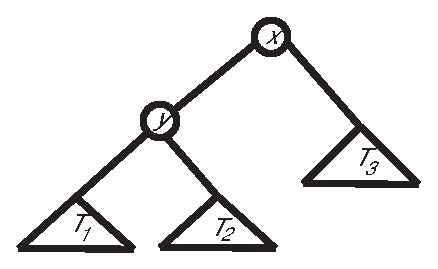
\includegraphics{pics/avl}
\caption{AVL strom}
\label{avltree}
\end{figure}

V tomto stromě jsou výšky podstromů $T_1$, $T_2$ a $T_3$ stejné. 
Pokud při vložení
nového vrcholu do podstromu T1 vzroste výška tohoto podstromu, bude vrchol
$x$ nevyvážený. Jeho vyvážení se však provede jednoduše pomocí 
tzv.~LL-rotace. (viz~obr.~\ref{avl-ll})

\begin{figure}[!htb]
\centering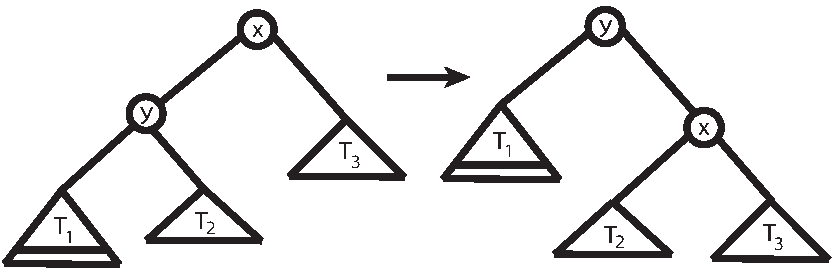
\includegraphics{pics/avl-ll}
\caption{LL-rotace pro AVL stromy}
\label{avl-ll}
\end{figure}

Pokud bychom však chtěli nový vrchol vložit do $T_2$ a výška tohoto podstromu
by vzrostla, byl by opět vrchol $x$ nevyvážený. To se může napravit pomocí
LR-rotace. (viz~obr.~\ref{avl-lr})

\begin{figure}[!htb]
\centering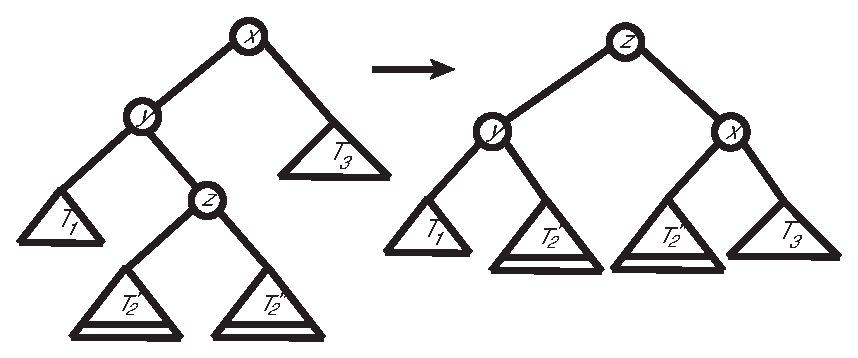
\includegraphics{pics/avl-lr}
\caption{LR-rotace pro AVL stromy}
\label{avl-lr}
\end{figure}

Poznamenejme, že na vyváženost nemá vliv, zda jsme vrchol vložili do
$T_{2}'$,
nebo do $T_{2}"$. Při vkládání nového vrcholu do pravého podstromu vrcholu
$x$ se pro vyvážení používají rotace RR-rotace a RL-rotace, které jsou 
symetrické k již uvedeným rotacím.

\begin{samepage}
LL-rotaci a RR-rotaci se také někdy říká jednoduchá rotace, kdežto
LR-rotaci a RL-rotaci se říká dvojitá rotace. Všimněte si, že po rotaci je
výška podstromu, se kterým se rotace prováděla, stejná jako jeho výška
před vložením nového vrcholu. Tedy po rotaci není narušena vyváženost
nějakého předka. Stačí tedy vyvážit ten nevyvážený vrchol, který je ve
stromu nejníže. Pokusme se nyní charakterizovat ten vrchol, který je třeba
vyvážit. Samozřejmě, že vrchol $x$ leží na cestě od kořene k přidanému
vrcholu a platí:
\begin{itemize}
\item buď $b(x)=1$ a nový vrchol je přidáván vlevo od $x$
\item nebo $b(x)=-1$ a nový vrchol je přidáván vpravo od $x$
\end{itemize}
\end{samepage}

Navíc pro každý vrchol $y$ na cestě od $x$ do přidaného listu je $b(y)=0$,
neboť jinak by byl sám nevyvážený, nebo by nezměnil svou výšku a tedy 
by nebylo třeba vyvažovat ani $x$.

Operace INSERT je formálně popsána algoritmem~\ref{alg:avl.ins}.

\begin{algorithm}[!htb]
\caption{INSERT pro AVL stromy}
\label{alg:avl.ins}
\begin{algorithmic}
\STATE INSERT($c$)
\STATE $r \leftarrow$ kořen
\WHILE {$r$ != NIL} 
\IF {$\text{prvek reprezentovaný } r = c$}
  \STATE END
\ENDIF
\IF {$balance(r)$ != $0$}
   \STATE $x := r$
\ENDIF
\IF {$\text{prvek reprezentovaný } r > c$}
  \STATE $r := left(r)$
\ELSE
  \STATE $r := right(r)$
\ENDIF
\ENDWHILE
\STATE \COMMENT {vložení nového vrcholu}
\STATE $r := \text{nový vrchol}$
\STATE $key(r):=c$
\STATE $b(r):=0$
\STATE $left(r):=nil$
\STATE $right(r):=nil$
\STATE $r:=x$
\STATE VYVAZUJ($r$)
\end{algorithmic}
\end{algorithm}


\begin{algorithm}[!htb]
\caption{VYVAZUJ pro AVL stromy}
\label{alg:avl.bal}
\begin{algorithmic}
\STATE \COMMENT {úprava balance (stačí od $x$ do vloženého listu)}
\WHILE {$r$ != NIL} 
  \IF {$\text{prvek reprezentovaný } r > c$}
        \STATE $balance(r) := balance(r) + 1$
        \STATE $r:=left(r)$
  \ENDIF
  \IF {$\text{prvek reprezentovaný } r < c$}
        \STATE $balance(r) := balance(r) - 1$
        \STATE $r := right(r)$
  \ELSE
        \STATE $r := NIL$
  \ENDIF
\ENDWHILE
\IF {$balance(x) = 2$}
  \IF {$\text{prvek reprezentovaný } left(x) > c$}
        \STATE LL-rotace
  \ELSE
        \STATE LR-rotace
  \ENDIF
\ENDIF
\IF {$balance(x) = -2$}
  \IF {$\text{prvek reprezentovaný } right(x) < c$}
        \STATE RR-rotace
  \ELSE
        \STATE RL-rotace
  \ENDIF
\ENDIF
\end{algorithmic}
\end{algorithm}



\subsection{Algoritmus DELETE}

Ubírání vrcholů z AVL-stromu se provádí stejně jako u nevyvážených
binárních vyhledávacích stromů. To znamená, že se ubíraný vrchol nahradí
nejpravějším vrcholem levého podstromu nebo nejlevějším vrcholem pravého
podstromu\footnote{To je klasický postup operace DELETE pro BVS popsaný
v~\cite{Topfer}, str.~70.}. 
Při tom se samozřejmě mohou také některé vrcholy stát
nevyváženými. To se opět řeší pomocí rotací.

\begin{algorithm}[!htb]
\caption{DELETE pro AVL stromy}
\label{alg:avl.del}
\begin{algorithmic}
\STATE DELETE($x$)
\STATE $r \leftarrow$ otec vrcholu reprezentovaného $x$
\STATE \COMMENT {vrcholu $left:=r$ jsme odebrali levého syna}
\WHILE {$r != NIL$}
\STATE \COMMENT {Prochází vrcholy od otce ubraného vrcholu ke kořeni}
  \IF {$left$}
        \IF {$b(r) = 0$}
		\STATE \COMMENT {Vrchol $r$ je stále vyvážený a výška jeho podstromu se nezměnila}
                \STATE $b(r) := -1$
        \ENDIF
        \IF {$b(r) = 1$}
		\STATE \COMMENT {Vrchol $r$ je stále vyvážený, ale výška jeho podstromu se snížila}
                \STATE $b(r) := 0$
	\STATE \COMMENT {Je třeba vyvažovat}
        \ELSE                            
                \STATE VYVAZUJ\_RIGHT(right($r$))
        \ENDIF
  \ELSE
        \IF {$b(r)=0$}
		\STATE \COMMENT {Vrchol $r$ je stále vyvážený a výška jeho podstromu se nezměnila}
                \STATE $b(r)=1$                  
                \STATE END
	\ENDIF
        \IF {$b(r)=-1$}
		\STATE \COMMENT {Vrchol $r$ je stále vyvážený, ale výška jeho podstromu se snížila}
                \STATE $b(r):=0$
		\STATE \COMMENT {Je třeba vyvažovat}
        \ELSE
		\STATE VYVAZUJ\_LEFT(left($r$))
        \ENDIF
  \ENDIF
\STATE $x:=r$
\STATE $r:=otec(r)$
\STATE $left:=left(r)=x$
\ENDWHILE
\end{algorithmic}
\end{algorithm}
%\end{samepage}

%\begin{samepage}
Operace DELETE je formálně popsána algoritmem~\ref{alg:avl.del}.
V algoritmu se používají dvě procedury pro vyvažování popsané v
algoritmech~\ref{alg:avl.del.vyvazuj.right}~a~\ref{alg:avl.del.vyvazuj.left}.

\begin{algorithm}[!htb]
\caption{VYVAZUJ\_RIGHT pro AVL stromy}
\label{alg:avl.del.vyvazuj.right}
\begin{algorithmic}
\STATE VYVAZUJ\_RIGHT(x)
\IF {$b(x) = 0$}
        \STATE RR-rotace
	\STATE END
\ENDIF        
		\STATE \COMMENT {Výška podstromu se nezměnila}
\IF {$b(x) = -1$}
        \STATE RR-rotace
\ELSE
        \STATE RL-rotace
\ENDIF
\end{algorithmic}
\end{algorithm}

\begin{algorithm}[!htb]
\caption{VYVAZUJ\_LEFT pro AVL stromy}
\label{alg:avl.del.vyvazuj.left}
\begin{algorithmic}
\STATE VYVAZUJ\_LEFT(x)
\IF {$b(x) = 0$}
        \STATE LL-rotace
		\STATE \COMMENT {Výška podstromu se nezměnila}
        \STATE END             
\ENDIF
\IF {$b(x) = 1$}
        \STATE LL-rotace
\ELSE
        \STATE LR-rotace
\ENDIF
\end{algorithmic}
\end{algorithm}
%\end{samepage}


%\begin{samepage}
Problém je, že ne při všech rotacích se zachovává výška podstromu, jak
tomu bylo u operace INSERT. Proto se zde vyvažování neomezí pouze na jeden
vrchol. Při operaci DELETE se může provést až $\log n$ rotací. Každopádně
složitost operace DELETE je stejně jako složitost operace INSERT $O(\log n)$.
\mnote{XXX dokázat max. počet rotací při DELETE}

% tohle by melo flushnout floats
% dalsi varianta:
% ctan macro/latex/contrib/supported/ placeins.sty 
% \floatbarrier command 
%\clearpage
\FloatBarrier

% --------------------------------------------------------------------------
\section{Červenočerné stromy}

\begin{defn}
Binární vyhledávací strom T se nazývá \emph{červenočerný}, jestliže každý 
vrchol je obarven červeně nebo černě a platí následující podmínky:
\begin{enumerate}
\item Listy jsou černé.
\item Pokud má červený vrchol otce, je otec černý.
\item Všechny cesty z kořene do listu mají stejný počet černých vrcholů.
\end{enumerate}
\end{defn}

\mnote{nejdelší cesta je max. 2$\times$ delší než nejkratší}

\begin{theorem} % XXX tvrzeni
Pro binární vyhledávací červenočerné stromy reprezentující množinu $S$,
$|S| = n$ platí, že jejich hloubka je $O(\log n)$.
\end{theorem}

\begin{proof}
je-li $k$ počet černých vrcholů na cestě z kořene do listu, pak
\[
2^k -1 \leq |S| \leq 2^{2k} -1
\]
To plyne z toho, že cesta z kořene do listu se může skládat v extrémních
případech buď z k černých vrcholů, pak je počet vnitřních vrcholů stromu
$1 + 2 + ... + 2^{k-1} = 2^k - 1$ nebo z cesty, kde se střídají černé a
červené vrcholy, pak je počet vnitřních vrcholů $1 + 2 + ... + 2^{2k-1} =
2^2k - 1$.
Tedy platí
\[
k \leq \log_2 |S| +1 \leq 2k
\]
přičemž prvky $S$ jsou reprezentovány pouze ve vnitřních vrcholech, ne
v listech. 
\mnote{to platí pro všechny bin. vyhl. stromy}
\end{proof}


\subsection{Operace INSERT}
Uvedeme pouze odlišnost od operace INSERT v obecném binárním
vyhledávacím stromě.

Situace: list $t$ se změnil na vnitřní vrchol reprezentující prvek $x$
a přidali jsme mu 2 listy.

Vrchol $t$ obarvíme červeně a jeho syny černě. Podmínky 1 a 3 stále
platí, ale podmínka 2 platit nemusí.
\begin{defn}
Strom a jeho vrchol $(T,t)$ nazveme \emph{2-téměř červenočerný strom
(2tččs),} jestliže platí
\begin{itemize}
\item{1} Listy jsou černé. {\it (nezměněno)}
\item{2'} Pokud má červený vrchol \emph{různý od $t$} otce, je otec
černý.
\mnote{Srovnej: Každý červený vrchol různý od $t$ má černého otce.}
\item{3} Všechny cesty z kořene do listu mají stejný počet černých
vrcholů. {\it (nezměněno)}
\end{itemize}
\end{defn}

\begin{defn}
Je-li vrchol $t$ červený a jeho otec je také červený, pak řekneme, že
$t$ je \emph{porucha}.
\end{defn}

\begin{pozn}
Poruše v 2tččs se také někdy říká \emph{2-porucha}.
\end{pozn}

Tedy nyní máme 2tččs $(T,t)$ Je-li $t$ porucha, pak ji musíme nějak
opravit. Situace je na obrázku~\ref{rbt-i}.

\begin{figure}[!htb]
\centering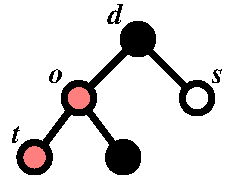
\includegraphics{pics/rbt-i}
\caption{Obecná situace při INSERTu}
\label{rbt-i}
\end{figure}

Nejprve záleží na tom, jakou barvu má $s$, strýc $t$:
\begin{enumerate}
\item $s$ je červený. Pak pouze přebarvíme $o$, $d$ a $s$ podle
obrázku \ref{rbt-i1}.
Podmínky 1 a 3 jsou splněny. Nyní $d$ může být porucha, ovšem posunutá o 2
hladiny výše. Vznikl 2tččs $(T,d)$.

\begin{figure}[!htb]
\centering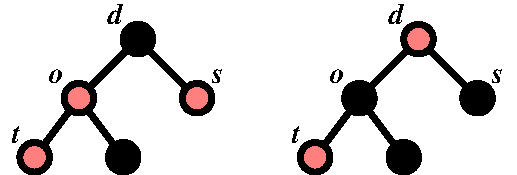
\includegraphics{pics/rbt-i1}
\caption{Oprava INSERTu přebarvením}
\label{rbt-i1}
\end{figure}

\item $s$ je černý. Záleží na tom, zda hodnota $t$ leží mezi hodnotami
$o$ a $d$ nebo ne. Jinými slovy, zda cesta $t$-$o$-$d$ obsahuje
\emph{zatáčku}.
\begin{enumerate}
\item Bez zatáčky:
Provedeme rotaci a přebarvíme podle obrázku \ref{rbt-i2a}.
Splněny budou podmínky 1, 2 i 3, tedy máme červenočerný strom.

\begin{figure}[!htb]
\centering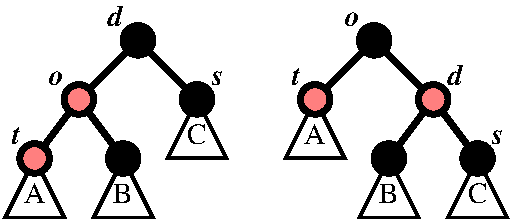
\includegraphics{pics/rbt-i2a}
\caption{Oprava INSERTu rotací a přebarvením}
\label{rbt-i2a}
\end{figure}

\item Se zatáčkou:
Provedeme dvojitou rotaci a přebarvíme podle obrázku \ref{rbt-i2b}.
Splněny budou podmínky 1, 2 i 3, opět máme rovnou červenočerný strom.

\begin{figure}[!htb]
\centering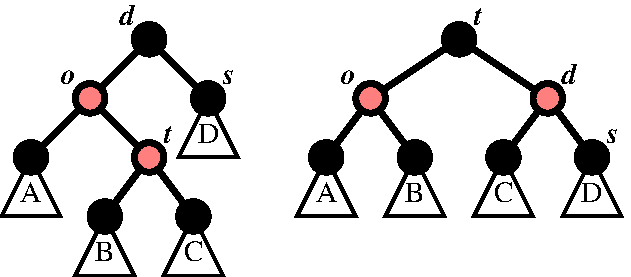
\includegraphics{pics/rbt-i2b}
\caption{Oprava INSERTu dvojitou rotací a přebarvením}
\label{rbt-i2b}
\end{figure}

\end{enumerate}
\end{enumerate}

\subsection{Operace DELETE}
Zatímco INSERT se příliš nelišil od své obdoby u AVL stromů, operace
DELETE u červenočerných stromů je oproti AVL stromům složitější
mentálně, ovšem jednodušší časově.

Situace: odstraňujeme vrchol $t$ (který nemusí reprezentovat
odstraňovaný prvek --- viz DELETE v obecných binárních vyhledávacích
stromech) a jeho syna, který je list.

Druhého syna $t$, $u$, dáme na místo smazaného $t$ a začerníme ho. Tím
máme splněné podmínky 1 a 2. Pokud byl ale $t$ černý, chybí nám na
cestách procházejících nyní vrcholem $u$ jeden černý vrchol.
\begin{defn}
Strom a jeho vrchol $(T,u)$ nazveme \emph{3-téměř červenočerný strom
(3tččs),} jestliže platí
\begin{itemize}
\item{1} Listy jsou černé. {\it (nezměněno)}
\item{2} Pokud má červený vrchol otce, je otec černý. {\it (nezměněno)}
\item{3'}
Všechny cesty z kořene do listu neprocházející $u$ mají stejný počet
černých vrcholů, nechť je to $k$. 
Všechny cesty z kořene do listu   procházející $u$ mají stejný počet
černých vrcholů, nechť je to $\ell$. 
A platí $k-1 \leq \ell \leq k$.
\end{itemize}
Když $u$ není kořen a $\ell < k$, pak řekneme, že $u$ je \emph{porucha}.
\end{defn}

\begin{pozn}
Takovému vrcholu v 3tččs se někdy říká \emph{3-porucha}.
\end{pozn}

Nechť vrchol $u$  je porucha. Pak můžeme předpokládat, že je 
obarven černě, jinak bychom ho přebarvili na černo a tím by se porucha 
odstranila a vznikl červenočerný strom.

Situace: máme 3tččs $(T,u)$, $u$ je porucha s otcem $o$, bratrem $b$ a
synovci $s1$, $s2$, viz obrázek \ref{rbt-d}.

\begin{figure}[!htb]
\centering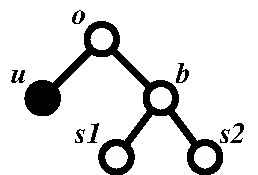
\includegraphics{pics/rbt-d}
\caption{Obecná situace při DELETE}
\label{rbt-d}
\end{figure}

\begin{samepage}
Oprava záleží na barvě vrcholu $b$:
\begin{enumerate}
\item Bratr je černý. 
Rozlišujeme dále 4 případy, z nichž jeden propaguje poruchu o hladinu
výš a ostatní skončí s červenočerným stromem.

\begin{enumerate}
\item Otec i synovci jsou černí.
Přebarvíme $b$ na červeno, viz obrázek \ref{rbt-d1a}. Dostáváme 3tččs $(T,o)$,
tedy porucha je o hladinu výše.

\begin{figure}[!htb]
\centering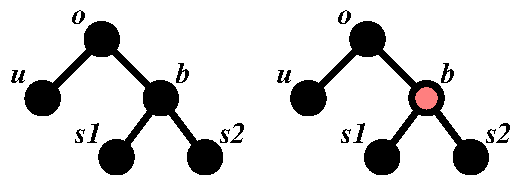
\includegraphics{pics/rbt-d1a}
\caption{Částečná oprava DELETE přebarvením}
\label{rbt-d1a}
\end{figure}
\item \label{rbt-cd1b} Otec je červený, synovci černí.
Přebarvíme otce a bratra podle obrázku \ref{rbt-d1b} a dostáváme
červenočerný strom.

\begin{figure}[!htb]
\centering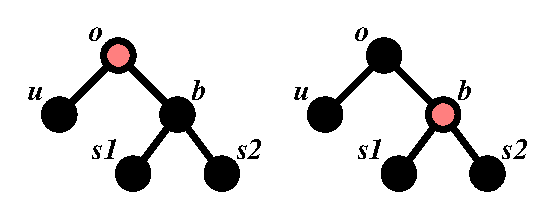
\includegraphics{pics/rbt-d1b}
\caption{Oprava DELETE přebarvením}
\label{rbt-d1b}
\end{figure}
\item \label{rbt-cd1c} Synovec $s1$, jehož hodnota leží mezi hodnotami
otce a bratra, je černý, druhý synovec je červený.
Přebarvíme a zrotujeme podle obrázku \ref{rbt-d1c}, barva otce se
nemění (tj., vrchol $b$ bude mít barvu, kterou původně měl vrchol $o$).
Dostáváme červenočerný strom.

\begin{figure}[!htb]
\centering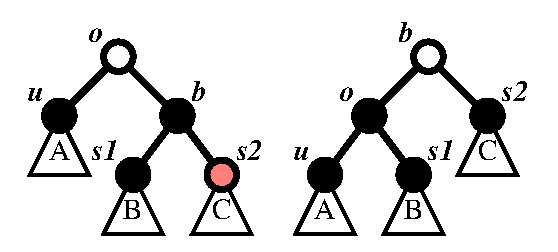
\includegraphics{pics/rbt-d1c}
\caption{Oprava DELETE přebarvením a rotací}
\label{rbt-d1c}
\end{figure}
\item \label{rbt-cd1d} Synovec $s1$, jehož hodnota leží mezi hodnotami
otce a bratra, je červený, druhý synovec má libovolnou barvu.
Přebarvíme a dvojitě zrotujeme podle obrázku \ref{rbt-d1d} (tj., vrchol $s1$ 
bude mít barvu, kterou původně měl vrchol $o$ a barva vrcholu $s2$ se nezmění).
Dostáváme červenočerný strom.

\begin{figure}[!htb]
\centering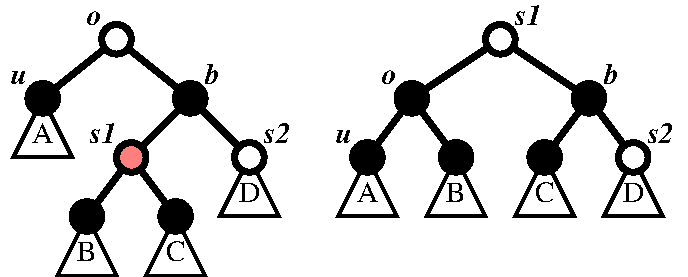
\includegraphics{pics/rbt-d1d}
\caption{Oprava DELETE přebarvením a dvojitou rotací}
\label{rbt-d1d}
\end{figure}

\end{enumerate}

\item Bratr je červený. Provedeme rotaci. 
Dostaneme strom ve tvaru, který je na \ref{rbt-d2}.
a aplikujeme předchozí případ č.1. \\
Přestože to tak na první pohled nevypadá, máme vyhráno, protože bratr 
poruchy je černý a otec červený, tedy příští oprava bude případ \ref{rbt-cd1b}, \ref{rbt-cd1c}, nebo \ref{rbt-cd1d} a skončíme s červenočerným 
stromem.

\begin{figure}[!htb]
\centering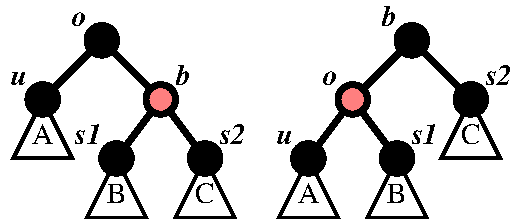
\includegraphics{pics/rbt-d2}
\caption{Částečná oprava DELETE přebarvením a rotací}
\label{rbt-d2}
\end{figure}

\end{enumerate}
\end{samepage}


\subsection{Závěry}
Pro binární vyhledávací červenočerné stromy lze implementovat MEMBER,
INSERT a DELETE tak, že vyžadují čas $O(\log n)$ a INSERT používá
nejvýše jednu (dvojitou) rotaci a DELETE používá nejvýše dvě rotace
nebo rotaci a dvojitou rotaci. 

Jsou lepší než AVL stromy, které při DELETE spotřebují až $\log n$
rotací. Oproti váhově vyváženým stromům i proti AVL stromům jsou 
červenočerné stromy jen
konstantně lepší, ale i to je dobré. Při použití binárních vyhledávacích 
stromů ve výpočetní geometrii nese informaci i rozložení prvků ve stromě, 
a tato informace se musí po provedení rotace nebo dvojité rotace aktualizovat. 
To znamená prohledání celého stromu a tedy čas $O(n)$ za každou rotaci a 
dvojitou rotaci navíc. Pro tyto problémy jsou červenočerné stromy obzvláště 
vhodné, protože minimalizují počet použitých rotací a dvojitých 
rotací\footnote{Červenočerné stromy se používají například ve 
\href{http://www.sgi.com/tech/stl/}%
standardní šablonové knihovně jazyka C++ od SGI, 
která je zahrnuta do GCC. Máte-li Linux, zkuste se podívat do
\path{/usr/include/g++-2/stl\_tree.h}; 
%pokud používáte OpenBSD, najdete
%implementaci jak červenočerných, tak splay stromů v
%\path{/usr/include/sys/tree.h}.
Co se týče "real-world" aplikací červeno-černých stromů, je možné zmínit
packet filter (PF) v OpenBSD, kde se tyto stromy používají k reprezentaci
pravidel pro firewall. Pro firewally je čas vyhodnocení jednotlivých
paketů proti pravidlům kritický. Zajímavé je, že původní implementaci PF
používala AVL stromy. Červeno-černé stromy se ukázaly jako výhodnější.
Implementaci červeno-černých stromů lze v OpenBSD najít v 
\path{/usr/include/sys/tree.h} v podobě maker jazyka C. Tento soubor 
obsahuje rovněž makra pro implementaci Splay stromů.
A pokud víte o podobně dostupných implementacích jiných
datových struktur z téhle přednášky, sem s nimi !}.

\begin{pozn}
Červenočerné stromy se používají při implementaci $(2,4)$-stromů, se
kterými se seznámíme v další kapitole. Vrchol 
se dvěma syny je nahrazen jedním černým vrcholem, vrchol se třemi syny 
je nahrazen černým vrcholem s jedním červeným synem a vrchol se čtyřmi 
syny je nahrazen černým vrcholem se dvěma syny. Pozor! Aktualizační 
operace pro $(2,4)$-stromy neodpovídají aktualizačním operacím na 
červenočerných stromech (i reprezentace prvků je odlišná).
\end{pozn}

